\documentclass[twoside, 12pt]{article}
%\usepackage{graphicx, xdipp,natbib}
% \usepackage{graphicx, xdipp, caption, parskip}
\usepackage{graphicx, xdipp, caption, listings, minted, float}

% \newcommand{\dummyfig}[3]{
%   \centering
%   \fbox{
%     \begin{minipage}[c][#2][c]{#3}
%       \centering{#1}
%     \end{minipage}
%   }
% }

\newfloat{listing}{htbp}{lop}
\floatname{listing}{Ukázka kódu}

\captionsetup[listing]{
  justification=raggedright,
  singlelinecheck=false       
}

% \lstset{
%   basicstyle=\ttfamily,
%   columns=fullflexible,
%   breaklines=true,
%   postbreak=\mbox{\textcolor{red}{$\hookrightarrow$}\space},
%   language=javascript,
%   frame=single
% }

% \newcommand{\charactercount}[1]{
% \immediate\write18{
%     expr `texcount -1 -sum -merge #1.tex` + `texcount -1 -sum -merge -char #1.tex` - 1 
%     > chars.txt
% }\input{chars.txt}}

% \pagestyle{plain}

\usepackage[style=iso-authoryear]{biblatex}
\addbibresource{BakalarkaZdroje.bib}
\usepackage{pdfpages}

\begin{document}

\titul{Webová aplikace pro podporu výuky 3D tisku}{Zdeněk Šilhán}{Ing. Robert Rouš}{Brno 2024}

\clearpage{\cleardoublepage\thispagestyle{empty}}

 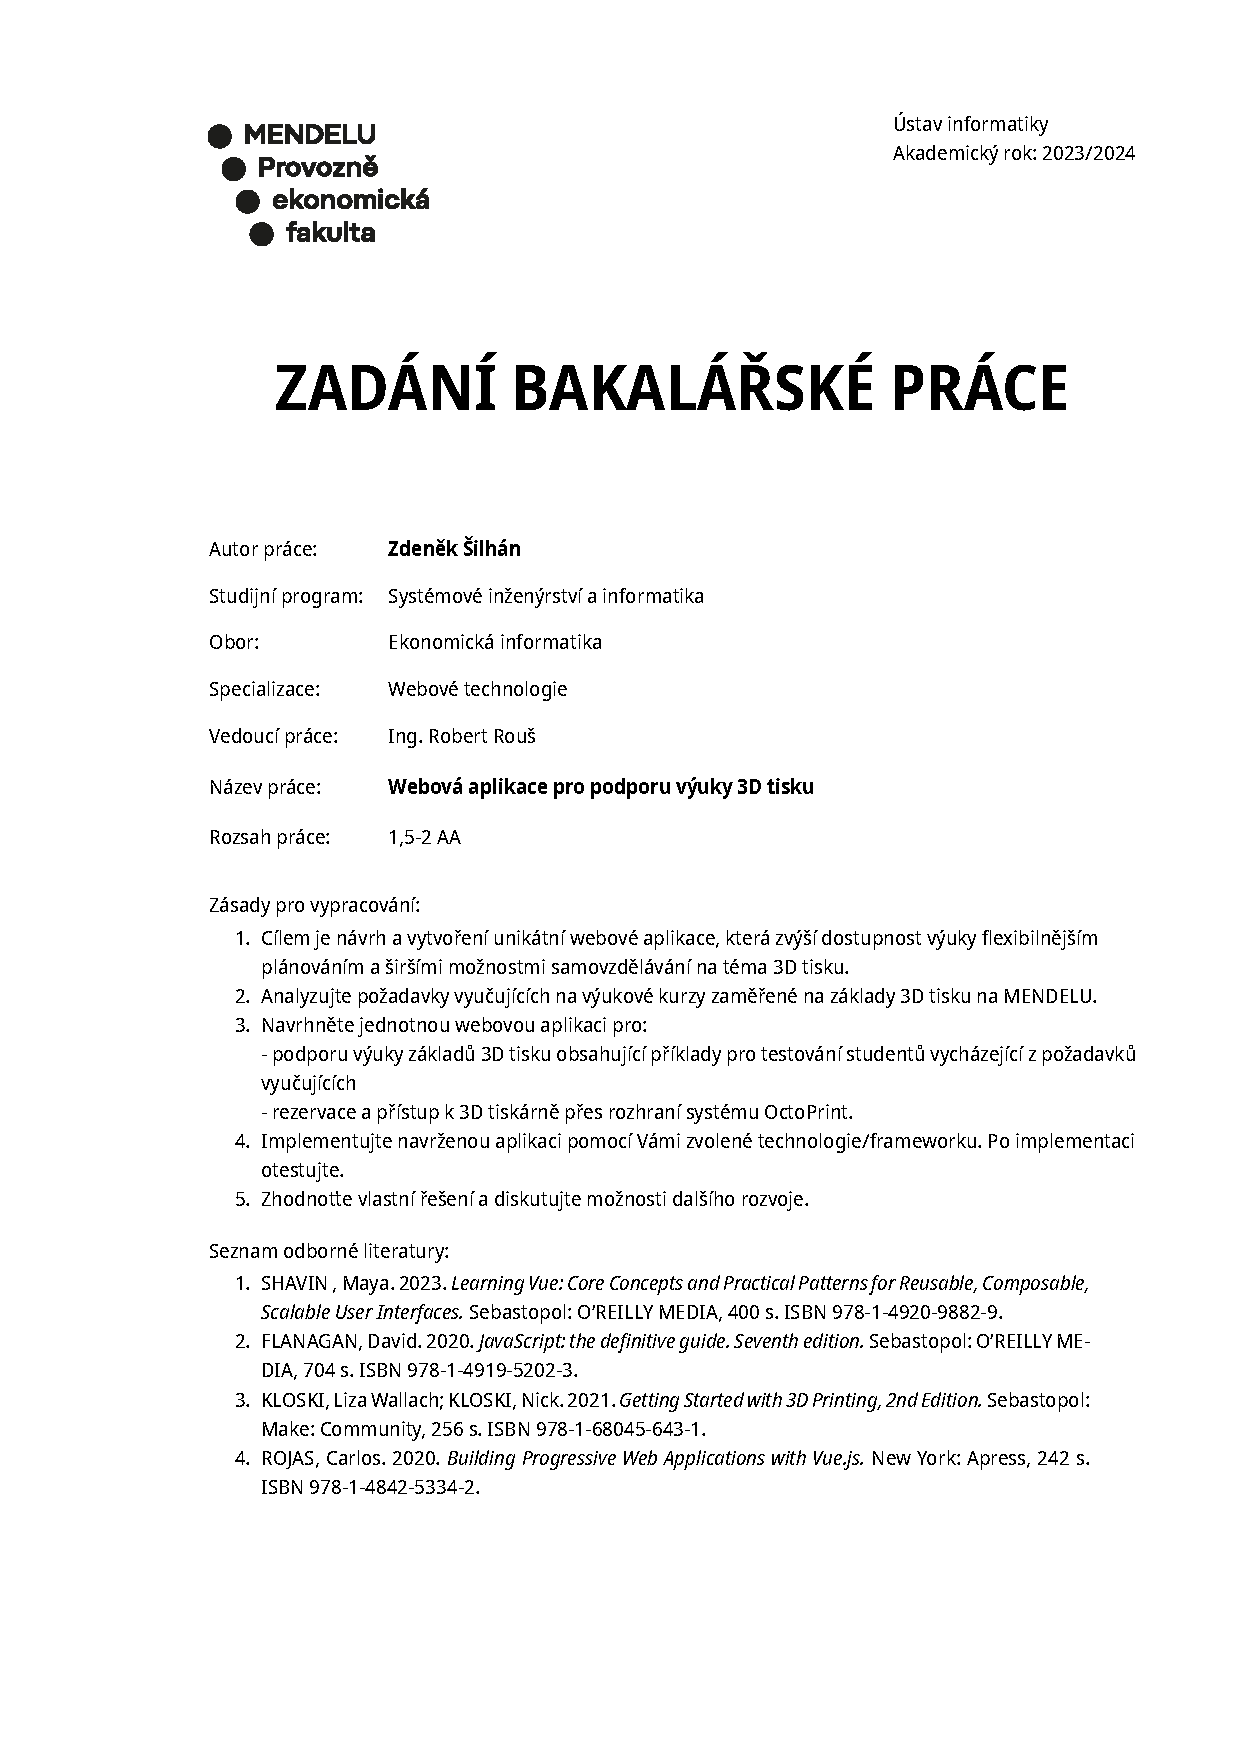
\includepdf[pages=-]{zadani.pdf}


% 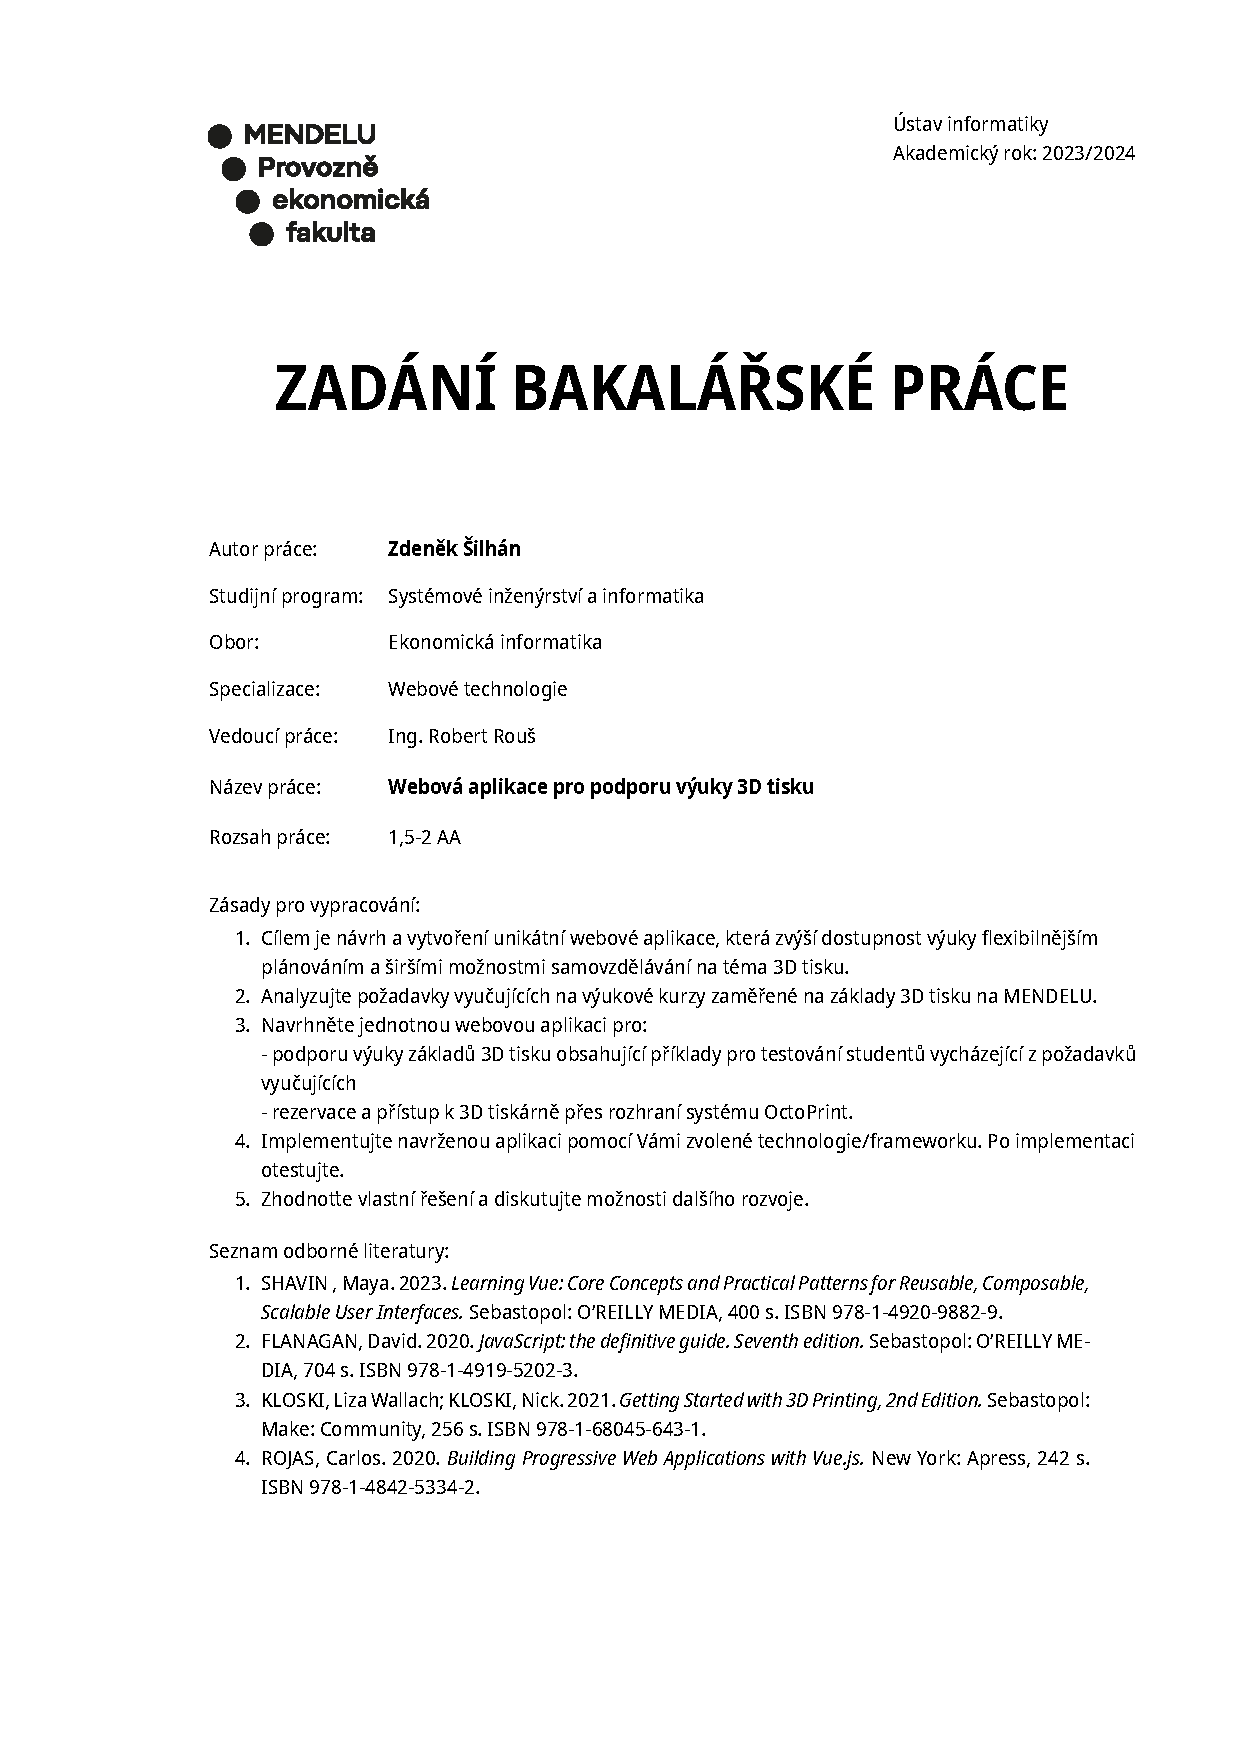
\includepdf{zadani.pdf}
% \includepdf{UseCase.pdf}

% \includegraphics{UseCase.pdf}

% \includepdf{}


\podekovani{Velké poděkování si zaslouží především Ing. Robert Rouš za vedení, trpělivost, rady a vyhrazený čas během psaní této bakalářské práce. Poděkování si zaslouží také Ing. Ivo Pisařovic, Ph.D., za návrh tématu a Bc. Jan Janča za pomoc při upřesnění požadavků. Dále bych chtěl poděkovat své rodině a přátelům za podporu a trpělivost.}



\prohlasenimuz{V Brně dne 12. května 2024}

\abstract{Šilhán, Z. Web application for 3D printing learning support. Bachelor thesis. Brno, 2024
}{The thesis deals with the design and implementation of a web application that aims to increase the accessibility of learning through more flexible scheduling and wider self-learning opportunities on the topic of 3D printing. It first introduces the used and related technologies and then deals with the analysis of the requirements of teachers from Mendel University in Brno. This is followed by the design of the user environment and the selection of appropriate teaching topics based on the analysis. This is followed by the implementation process utilizing Vue, Vuetify, Node, Express, SQLite and then concludes with a discussion on possible extensions and improvements.}
\keywords{JavaScript, Vue.js, OctoPrint, web application, 3D printing, educational application, reservation system, gamification}

\abstrakt{Šilhán, Z. Webová aplikace pro podporu výuky 3D tisku. Bakalářská práce. Brno, 2024
}{Práce se zabývá návrhem a implementací webové aplikace, jejímž cílem je zvýšení dostupnosti výuky flexibilnějším plánováním a širšími možnostmi samovzdělávání na téma 3D tisku. Nejprve představuje použité a související technologie a poté se zabývá analýzou požadavků vyučujících z Mendelovy univerzity v Brně. Následuje návrh uživatelského prostředí a zvolení vhodných výukových témat na základě analýzy. Dále je popsán proces implementace aplikace za použití Vue, Vuetify, Node, Express, SQLite a práce je zakončena diskusí na téma možného rozšíření a vylepšení.}

\klslova{JavaScript, Vue.js, OctoPrint, webová aplikace, 3D tisk, výuková aplikace, rezervační systém, gamifikace}



\obsah



\kapitola{Úvod a cíl práce}
\sekce{Úvod}
I když se první myšlenky popisující základní principy fungování 3D tisku začaly objevovat během pozdních 40. let 20. století, tak posun k prakticky použitelné technologii trval až do 80. let. Velký zlom v cenové dostupnosti 3D tiskáren nastal až na začátku 21. století a zasloužily se o něj především tiskárny využívající technologii FDM,\footnote{Fused Deposition Modeling je způsob výroby, při kterém dochází k tavení polymeru skrze trysku na tiskovou plochu, kde následně chladne.} která je v současné době nejpoužívanější především kvůli dostupnosti a široké nabídce materiálů, které jsou dostačující pro běžného spotřebitele. (\cite{FDMmarketShare}) Jak se tyto aditivní technologie výroby stávají čím dál běžnější součástí různých odvětví od průmyslové výroby až po kreativní činnosti, tak vyvstává potřeba předávat znalosti dalším generacím. Zde nastává hlavní problém. Jak motivovat žáky k prohloubení znalostí zdánlivě technicky velmi složitého oboru? Možným pomocníkem by se mohla stát aplikace, která umožní učiteli efektivněji vést výuku vytvářením kvízů, návodů a zjednodušením procesu tvorby rezervací 3D tiskárny pro jednotlivé žáky i mimo výuku, současně pomůže s motivováním žáků k aktivní účasti pomocí gamifikačních prvků, statistik a systému odměn.

\sekce{Cíl}

Cílem je návrh a vytvoření unikátní webové aplikace, která sníží administrativní zátěž kladenou na učitele, zvýší dostupnost výuky flexibilnějším plánováním a širšími možnostmi samovzdělávání na téma 3D tisku. Uživatelské prostředí bude navrženo intuitivně, aby se v něm dokázal zorientovat a efektivně ho používat i laik. Konečným cílem je předání fundamentálních znalostí o 3D tisku zajímavou formou a taktéž zajištění plynulého fungování a spravování přístupu k samotné 3D tiskárně.
				
\kapitola{Rešerše}

\sekce{Přehled existujících řešení}

\podsekce{Sdílený kalendář}

Řada institucí využívá pro rezervace sdílený kalendář. Nejčastěji se lze setkat s kalendářem od firmy Google, který nabízí velmi jednoduché sdílení vytvořeného kalendáře velkému množství žáků bez nutnosti instalace speciálních aplikací a dokáže uživateli zprostředkovat i notifikace na mobilních zařízeních upozorňující na nadcházející rezervace. Na obrázku níže můžeme vidět řešení využívané na Lawrence University ve Spojených státech amerických. Univerzita tam nabízí k rezervaci celkem čtyři 3D tiskárny a každá má svůj vlastní kalendář. Obdobně je řešena i rezervace šicích strojů a laserové řezačky.

\obrazek
     \vlozobrbox{obrazky/google kalendar rezervace.png}{.7\textwidth}{!}
     \endobrl{Sdílený Google kalendář: Lawrence University \obrzdroj{https://www.lawrence.edu/}}{GoogleKal}



\podsekce{Sdílený dokument}
Poněkud primitivnějším způsobem je vytvoření dokumentu, ve kterém se uživatelé registrují zapsáním do příslušné kolonky. Tento způsob využívá například School of Architecture University of Miami, která takto spravuje čtyři 3D tiskárny současně v jednom Google sheet dokumentu. Přehlednost tohoto dokumentu je přinejlepším mizivá a neexistuje žádný způsob zajištění notifikaci na nadcházející rezervace.

\obrazek
     \vlozobrbox{obrazky/excel rezervace.png}{.7\textwidth}{!}
     \endobrl{Sdílený dokument: School of Architecture, University of Miami \obrzdroj{https://umddw.wordpress.com/}}{Excel}



\podsekce{Rezervační systém}

Nejvhodnějším řešením je využití rezervačního systému, který oproti předešlým způsobům nabízí přehlednost, škálovatelnost a možnost řešení přímo na míru. Velkou výhodou rezervačního systému na míru jsou široké možnosti využití a zobrazení dat, která vznikají provozem systému a na jejichž základě jsme schopni získat určitý vhled do chování uživatelů a činit podložená rozhodnutí. Řada firem nabízí již hotová univerzální řešení jako třeba Skedda,\footnote{Dostupné na: https://www.skedda.com/} zde ovšem narážíme na problém nenulové ceny v kombinaci s nedokonalým uzpůsobením potřebám 3D tisku. Na obrázku č. \ref{knihovna3} je vyobrazen rezervační systém používaný pro správu veřejné 3D tiskárny umístěné v knihovně města Wilmington.



\obrazek
\vlozobrbox{obrazky/Rezervacni system.png}{.7\textwidth}{!}
\endobrl{Rezervační systém: Wilmington Memorial Library \obrzdroj{https://wilmlibrary.org/}}{knihovna3}


\sekce{Technologická rešerše}

\podsekce{Základy webových technologií}

\textbf{HTML}

Hypertext Markup Language vznikl už v roce 1990 a představuje základní stavební kámen webu, který se stará o obsah a strukturu webové stránky. Jedná se o značkovací jazyk, který při tvorbě stránek využívá propojení hypertextovými odkazy a systémů značek (tagů), jež jsou zobrazovány s jejich předdefinovanými vlastnostmi. Standard HTML je spravován a vyvíjen komunitou WHATWG\footnote{Web Hypertext Application Technology Working Group je skupina pracující především na vývoji standardu HTML.} a W3C\footnote{World Wide Web Consortium je mezinárodní nezisková organizace spolupracují na vývoji standardů pro web.} (\cite{W3CWHATWG}). Velkou výhodou oddělení obsahu a struktury od vizuálu je možnost prezentovat čistý obsah jednodušeji například osobám se zrakovým postižením, pro které graficky složité stránky často představují překážku, jelikož nemusí být dobře kompatibilní s jejich čtečkou. Pro tvorbu vizuálně zajímavých stránek se zpravidla používá v kombinaci s CSS.

Nejnovější verze HTML5, vydaná koncem roku 2014, přináší zvýšení přehlednosti kódu, čehož je docíleno novou skupinou tagů, perzistentním úložištěm, podporou pro offline aplikace, API pro složitější webové aplikace a řadou optimalizací pro mobilní zařízení (\cite{HTMLinfo}). Od verze 5.1 je součástí standardu HTML i kontroverzní poloproprietární Encrypted Media Extension, které přidává nativní podporu pro přehrávání šifrovaného obsahu ve snaze o omezení stahování nebo kopírování obsahu, ke kterému legálně nevlastníte dešifrovací klíč. Jedná se tedy efektivně o DRM\footnote{Digital Rights Management slouží ke kontrole distribuce licencovaného obsahu.} ochranu, o jejíž přidání dlouho usilovala řada streamovacích služeb, jako je například Netflix, HBO nebo Disney+. (\cite{HTMLdrm})
\\
\\
\textbf{CSS}

Cascading Style Sheets, spravovaný taktéž organizací W3C, je jazyk sloužící pro pro definici vizuální stránky elementů, zejména v dokumentech zapsaných ve značkovacích jazycích jako HTML, XML atd. Myšlenkou je oddělení vzhledu od struktury a obsahu, což poskytuje mnohem širší možnosti modifikace vizuálu bez zásahu do struktury stránky a naopak. CSS vývojáři nabídne možnost si definovat vzhled, ať už se jedná o velikost písma, barvu textu, pozice na stránce, či nadřazený element.

Za původním návrhem CSS v roce 1996 stal Håkon Wium Lie, který se i nadále podílí na rozvoji webu skrz své působení v organizaci WHATWG. CSS je v současné době ve verzi CSS3, která se úzce pojí se standardem HTML5 a přináší širší možnosti úpravy vzhledu, animace elementů, automatické vícesloupcové rozvržení, robustnější pravidla pro přetékání atd. (\cite{CSS3})




\podsekce{Frontend webové technologie}

Volba vhodného frontendového frameworku či knihovny je klíčová pro celkový zážitek z užívání aplikace. Na rozdíl od uživatelsky neviditelného backendu má frontend přímý dopad na to, jak uživatelé vnímají a interagují s webovou aplikací. Frontend udává vzhled, responzivnost a líbivost celé webové aplikace. Jelikož nedesignujeme aplikací pro roboty, ale pro lidské bytosti plné emocí, dojmů a předsudků, které jsou neúměrně ovlivněni prvním dojmem, je proto potřeba této části věnovat extra pozornost. Pro vývojáře bude zase klíčové, zda je daný framework vhodný pro zamýšlenou webovou aplikaci. Dalšími parametry ke zvážení může být množství dostupných učebních materiálů, velikost komunity, kompatibilita a snadnost integrace s dalšími knihovnami, rychlost vývoje a především budoucí udržitelnost.
\\
\\
\textbf{Vue.js}

Vue.js je progresivní JavaScript framework, který má své kořeny v roce 2014. Za svůj vznik vděčí Evanovi You, který se po dřívější zkušenosti s frameworkem Angular během jeho práce pro Google rozhodl vytvořit nový lehký framework. Ten se v lecčem inspiroval Reactem i Angularem, ale zároveň si zakládá na své jednoduchosti, díky čemuž v benchmarcích dosahuje rychlostního náskoku oproti jeho největším rivalům (\cite{VueRychlost}). Je důležité zmínit, že se jedná o nezávislý open-source projekt, který je udržován jak týmem dedikovaných core team „zaměstnanců“, tak i řadou dobrovolníků z celého světa. V současné době koexistují Vue 2 a Vue 3, i když pouze pozdější verze 3 je v současné době aktivně vyvíjena. Část nových funkcí z Vue 3 byla přidána i do Vue 2.7, ale i tak je doporučeno provést migraci na Vue 3 do začátku roku 2024, kdy dojde k ukončení osmnáctiměsíční podpory od vydání Vue 2.7 z června roku 2022. Vue jako takové je implementované v TypeScriptu, ale jeho využití není vynuceno a vývoji v JavaScriptu nic nebrání. Oproti ostatním frameworkům kromě rychlosti Vue zaujme možností velmi rychle a efektivně vytvářet webové aplikace s využitím reactive data binding, oficiálního Vue routeru, computed properties a velmi užitečných DevTools. (\cite{Shavin2023}) Z tradičních návrhových vzorů je nejvíce inspirováno MVVM\footnote{Model-View-ViewModel je softwarový architektonický vzor, který odděluje aplikaci na tři oddělené části: správu dat, uživatelské rozhraní a jejich propojení skrze ViewModel.} modelem, ale samotné Vue.js je zaměřeno především na ViewModel.

Vue.js staví na systému znovupoužitelných komponent, kde každá komponenta má svoji šablonu obsahující styl spolu s logikou. Tyto komponenty jsou uspořádány do stromu komponent. Používá se i jednosměrného toku dat, kdy dochází k předávání pouze z rodičovských komponent do dceřiných, což vede k výraznému zjednodušení správy kódů a debugování. Za ocenění rozhodně stojí i oficiální dokumentace, která je často chválena pro svou jednoduchost a srozumitelnost. (\cite{VueDokumentace})
\\
\\
\textbf{Angular}

Jedná se o platformu a FOSS\footnote{Free and open-source software, jehož zdrojový kód je volně dostupný k nahlédnutí, úpravě a užívání. (\cite{FOSS})} framework umožňující tvorbu single-page aplikaci s využitím HTML a TypeScriptu. Hlavními stavebními bloky jsou znovupoužitelné izolované komponenty a služby sloužící pro komunikaci a distribuci dat v rámci aplikace.

Oproti předchůdci AngularJS se Angular liší využitím TypeScriptu oproti původnímu JavaScriptu, změnou syntaxe a hierarchii komponent. I když za Angularem stojí obří korporace, kterou je Googlu, tak jeho vývoj zůstává společnou snahou Googlu a open-source komunity. Aktualizace se vydávají 2× ročně a podpora trvá 18 měsíců. Mezi velké milníky vývoje patří přidání podpory pro PWA\footnote{Progressive web apps nabízejí uživatelský zážitek blízký nativním aplikacím.} ve verzi 5 nebo AOT\footnote{Ahead-of-time compilation kompiluje vysokoúrovňový kód do strojového ještě před spuštěním.} kompilace pro snížení zátěže na mobilní zařízení při run time. (\cite{AngularAbout})
\\
\\
\textbf{Svelte}

Svelte je nástroj pro tvorbu komponent uživatelského rozhraní a zároveň i programovací jazyk, za jehož vznikem stojí Rich Harris. Přístup Sveltu je rozdílný v tom, že napsaný kód zkompiluje do čistého JavaScriptu bez použití virtuálního DOM\footnote{Document Object Model je rozhraní umožňující změny struktury, stylu a obsahu webových stránek.} jako například React nebo Vue, což značně usnadňuje práci prohlížeče a zrychluje celou aplikaci. (\cite{Svelte}) Svelte byl pro svůj neobvyklý přístup a uživatelskou přívětivost zvolen jedním z nejvíce obdivovaných jazyků a zároveň se těší velké oblibě a zájmu mezi vývojáři, kteří s ním začínají nebo ho ještě nezkusili (\cite{SvelteSurvey}).
\\
\\
\textbf{React}

React, také známý jako React.js či ReactJS, je frontendovou JavaScript knihovnou, za jejíž vznikem stojí Facebook (nyní Meta). Je vyvíjen ve spolupráci Mety, dalších firem i individuálních vývojářů. React je vhodný pro vývoj mobilních, single page i SSR\footnote{Server-side rendering je technika, při které se aplikace vykreslují na serveru, nikoli na zařízení uživatele.} aplikací. React umožňuje vytváření uživatelských rozhraní pomocí skládání individuálních znovupoužitelných komponent, a jelikož využívá deklarativní přístup, tak má programátor přesnou kontrolu nad každou komponentou a takový kód je pak předvídatelnější a lehčí na debugování. Mezi hlavní výhody Reactu patří fakt, že znovu renderuje jen ty části stránky, kde došlo ke změně dat. Toho je docíleno pomocí virtuálního DOM (jedná se o odlehčenou kopii reálného DOM), který se updatuje ihned po změně stavu komponenty a následně proběhne porovnání s předchozí verzí virtuálního DOM a tyto změny jsou co nejefektivněji přeneseny i do reálného DOM, často se tento proces „dávkuje“, aby se zamezilo zbytečnému přepisování reálného DOM při sebemenší změně, což by znamenalo značné snížení výkonu. (\cite{React})

Další zajímavou vlastností je použití JSX,\footnote{JavaScript XML je syntaktické rozšíření JavaScriptu.} díky čemuž je umožněno psaní kódu a struktur velmi podobných HTML uvnitř JavaScriptových souborů, což značně zvyšuje vývojářský komfort a nabízí kontrolu syntaktických chyb v JSX při kompilaci. (\cite{ReactJSX})
\\
\\
\textbf{Vuetify}

Vuetify je komponentový framework pro Vue.js nabízející celou řadu znovupoužitelných, předvytvořených komponent vyvedených ve stylu Material Design (\cite{VuetifyMaterialDesign}), které umožňují vývojářům rychle vytvořit moderně vypadající, konzistentní a reaktivní web aplikace založené na Vue.js. Kromě širokého výběru tlačítek, kartiček, dialogů, navigačních lišt atd. je Vuetify velmi nápomocné při vytváření přístupného webu pro každého uživatele, jelikož splňuje WCAG\footnote{Web Content Accessibility Guidelines je sada doporučení pro zvýšení přístupnosti webového obsahu.} standardy, díky čemuž i uživatel se smyslovým postižením nebude připraven o možnost konzumace obsahu a využívání funkcionalit webové aplikace. Vedle skvělé podpory pro osoby s postižením nabízí Vuetify i širokou podporu od své komunity, která pravidelně vydává aktualizace. Vuetify disponuje i komponentovou knihovnou pro designový nástroj Figma,\footnote{Dostupné na: https://www.figma.com/} což usnadní tvorbu uživatelského rozhraní v počátečních fázích vývoje. Nevýhodou může být dočasné přechodné období z Vuetify 2.0, kompatibilním s Vue 2, na Vuetify 3.0, určeným pro Vue 3. I když byla verze 3.0 vydána v říjnu roku 2022, tak podle oficiálních stránek stále nezahrnuje všechny komponenty dostupné ve verzi 2.0. Naštěstí je řada z nich dostupná přes Vuetify Labs, ale zde je nutné zmínit, že se nejedná o produkční verzi komponent, a není tedy zcela vhodné je používat, pokud existuje vhodné alternativa. (\cite{VuetifyAbout})




\podsekce{Backend webové technologie}
Při výběru backend frameworku bereme zřetel čistě na technické fungování a preferovaný programovací jazyk. Ale ani zde samozřejmě nenalézáme univerzální řešení pro všechny situace. Přístupy jsou rozdílné, takže jeden framework vám může nabídnout všeobecně standardizovaný postup pro implementaci autentizačních služeb, middlewaru, databáze a přístupu, díky čemuž vývojáři na jednu stranu šetří čas, ale zároveň mají svázané ruce, pokud v průběhu vývoje vznikne nutnost použít funkcionality, které nejsou dostupné nebo jsou jen obtížně implementovatelné s využitím standardizovaného přístupu daného frameworku. (\cite{BEbasic2})
\\
\\
\textbf{Node.js}

Node.js je určen pro vytváření velmi dobře škálovatelných síťových aplikací starajících se o obří objemy dat s nízkou latencí. Jak už název napovídá programovacím jazykem je zde JavaScript, což může být nezanedbatelná výhoda jednotného jazyka pro serverovou i klientskou část. Jelikož se jedná o asynchronní běhové prostředí, tak velmi efektivně zvládá zpracování více požadavků současně, čímž výrazně zvyšuje výkon pro aplikace, u nichž je minimální odezva a vysoká propustnost klíčová. (\cite{NodeAbout}) Nikoho tedy nepřekvapí, že mezi společnosti využívající Node.js se řadí například Netflix (\cite{NodeNetflix}), Uber a PayPal. I když je Node.js navržen bez vláken, tak je schopen pomoci child procesu nebo modulu cluster rozložit zátěž na teoreticky neomezený počet jader/vláken. Prakticky ale vzniká režie správou child procesů a komunikace mezi nimi a v určitém momentě zvýšení počtu child procesu bude přinášet čím dál menší zvýšení výkonu. (\cite{NodeScalability})
\\
\\
\textbf{Express.js}

Jedná se o velmi minimalistický framework pro tvorbu webových aplikací, HTTP serveru, SPA\footnote{Single Page Application načítá jedinou HTML stránku a upravuje ji podle interakci uživatele.} nebo Microservices založených na Node.js. Urychluje a zjednodušuje vývoj díky přítomnosti middleware, což umožňuje vykonávat úkoly nad request a response objekty. Příkladem může být autentizace a autorizace skrz middleware express-jwt,\footnote{Dostupné na: https://www.npmjs.com/package/express-jwt} který používá JSON Web Token pro jednodušší a robustnější bezstavové zabezpečení. Jelikož Express.js staví na asynchronní nátuře Node.js, je schopen nabídnout velmi dobrou rychlost I/O operací i HTTP requestu. Express obsahuje i robustní router, který podporuje moderní funkce jako parametry přímo v URL adrese. Stejně jako v případě Node.js je zde programovacím jazykem JavaScript. (\cite{Express})
\\
\\
\textbf{Spring}

Od svého založení v roce 2002 umožňuje jeho flexibilní architektura zajišťovat provoz systémů různých velikostí, od malých po velké enterprise aplikace. Jedná se o velmi rozsáhlý webový framework, který vývojáři nabízí už hotová řešení pro celou škálu běžných problémů. Mezi webovými frameworky využívajícími Javu se jedná o nejpoužívanější s velkým předstihem (\cite{SpringSurvey}). Obsahuje celou řadu modulů, mezi které patří například Spring Boot pro výchozí konfigurace, Spring Data pro integraci s relačními a NoSQL\footnote{Not Only SQL je kategorie databází, která nabízí flexibilitu při práci s různými typy dat.} databázemi, Spring Security starající se o autentizaci a autorizaci uživatelů. Vývojáři je ponechána možnost vybrat si které moduly jsou vhodné pro jeho projekt, a zbytek nepoužít, čímž se vyvaruje vytvoření těžkého, pomalého monolitu. (\cite{SpringModuly})
\\
\\
\textbf{Flask}

Flask je velmi minimalistický webový micro framework využívající Python jako programovací jazyk. Používá šablonovací systém Jinja2,\footnote{Dostupné na: https://github.com/pallets/jinja} vycházející ze syntaxe frameworku Django. Flask jako takový nenabízí řadu funkcí jako snadnější integraci databáze nebo zpracování formulářů. Tato zdánlivá nevýhoda je ovšem nulována podporou rozšíření, které tuto chybějící funkcionalitu doplní. Mezi populární rozšíření patří Flask-SQLAlchemy pro objektově relační mapování nebo Flask-WTF pro tvorbu a validaci dat z formulářů od uživatele. (\cite{FlaskKnizka}) I když se jedná v základu o velmi omezený framework, tak podpora rozšíření a velká komunita z něj dělá po boku Djanga jeden z nejoblíbenějších webových frameworků pro Python (\cite{PythonSurvey}).
\\
\\
\textbf{Django}

Jedná se o další webový framework pro programovací jazyk Python, ale na rozdíl od Flasku nabízí mnohem komplexnější funkcionality bez nutnosti rozšíření. V praxi to vypadá tak, že v základu nabídne ORM\footnote{Object-Relational Mapping umožňuje mapovat objekty v OOP na tabulky v relační databázi.} nebo například ochranu proti SQL injection nebo cross-site scripting. Základním principem je Don't Repeat Yourself, který cílí na minimalizaci opakování kódu pomocí abstrakce do znovupoužitelných komponent, což činí kód čistší a snadněji udržitelný. Vhodné je zmínit i vestavěné webové admin rozhraní, skrz které lze rychle a efektivně spravovat databáze přímo z prostředí webového prohlížeče. (\cite{Django})
\\
\\
\textbf{Laravel}

Laravel je moderní open-source framework pro vývoj webových aplikací využívající MVC\footnote{Model–View–Controller návrhový vzor rozdělující aplikaci do tří hlavních komponent.} architekturu, programovacím jazykem je PHP a jeho první verze vyšla roku 2011. Mezi nejvíce oceňované součástí Laravelu patří Eloquent, jedná se o ORM nástroj pro konverzi entit v relační databázi do instancí tříd v objektově orientovaném programování. (\cite{Laravel})

\podsekce{Shrnutí technologické rešerše}

Na základě rešerše se jako nejvhodnější kombinace jeví Vue.js v kombinaci s komponentovým frameworkem Vuetify. Nabídnou velmi rychlý a efektivní vývojový proces, vysoký výkon, konzistentní a moderní uživatelské prostředí ve stylu Material Design, které je ale zároveň velmi dobře přístupné uživatelům se zrakovým či pohybovým postižením. Kromě výše zmíněných důvodů hraje roli i má osobní zkušenost s těmito frameworky a taktéž velmi dobře zpracovaná dokumentace Vue.js.

Díky zvolení JavaScript frontend frameworku byla vysoká preference pro backend framework také využívající JavaScript, jelikož tato volba výrazně usnadní komunikaci či umožní sdílet části kódu mezi klientskou a serverovou částí aplikace a napomůže snadnější údržbě.  (\cite{Flanagan2020}) Vybrán byl Express.js pro svoji rychlost, popularitu a podporu pro velmi dobrý autentizační middleware. Vue.js i Express.js sdílí stejný manažer balíčků npm,\footnote{Node Package Manager je manažer balíčků pro ekosystém postavený na nebo okolo Node.js. Může sloužit i jako lokální dependency manager pomocí package.json souboru.} který poskytuje širokou škálu dalších nástrojů a knihoven pro následný vývoj nových funkcionalit a zlepšení aplikace.


\podsekce{Jazyky}
Předchozí výběr frontend a backend frameworku určil programovacím jazykem webové aplikace JavaScript. Není náhodou, že od svého vzniku v roce 1995 se stal velmi důležitou součástí moderního interaktivního webu po boku HTML a CSS. Vzhledem k jeho popularitě a rozšířenému používání bylo nezbytné zavést základní standardizaci, která by zaručila vzájemnou kompatibilitu mezi prohlížeči. Tímto standardem je ECMAScript, který definuje jednotné specifikace pro JavaScript. Proces zobrazení webové stránky využívající JavaScript zahrnuje kompilaci kódu javascriptovým enginem prohlížeče do nativního strojového kódu těsně před spuštěním, což zajistí maximální možný výkon a díky dodržování standardů ECMAScript také zaručuje kompatibilitu napříč různými prohlížeči. (\cite{Flanagan2020})

\podsekce{Databáze}

Databáze byla zvolena SQLite pro svou jednoduchost a velmi dobrou přenositelnost mezi platformami. Jedná se o nejpoužívanější databázový systém na světě. Celá databáze se ukládá do jediného souboru, což je důvodem špatného škálování výkonu s větším počtem dat, a tudíž je SQLite vhodné spíše pro aplikace s menšími datovými požadavky a nízkou frekvencí zápisu nebo čtení z databáze. SQLite nevyžaduje běžící databázový server a její zdrojový kód je open-source. (\cite{SQLite})

\clearpage
\podsekce{Relevantní technologie}

K vypracování této práce nestačily pouze znalosti z oblasti webových technologií, ale bylo potřeba se seznámit s celou řadou dalších oblastí, které si stručně shrneme v následujících podkapitolách.
\\
\\
\textbf{3D tisk}

Jedná se o aditivní způsob výroby, tedy postupné přidávání materiálu vrstvu po vrstvě na základě 3D modelu, dokud nevznikne požadovaný objekt. Využití nachází 3D tisk především v odvětvích vyžadujících rychlé prototypování, umění, lékařství a v samotné výrobě. Mezi komerčně nejpoužívanější řadíme Fused Deposition Modeling (FDM), Stereolithography (SLA) a Selective Laser Sintering (SLS). Každá z těchto technologií nabízí řadu výhod, nevýhod, dostupných materiálů, rozdílných cenových hladin oproti ostatním, a žádná se tedy nedá univerzálně označit za nejlepší. (\cite{Zaklady3Dtisku})

\begin{itemize}
    \item \textbf{FDM} -- Nejběžnější technologie 3D tisku, zejména díky své velmi dobré dostupnosti a nízkým nákladům. Pracuje na principu protlačování nataveného polymeru tryskou na tiskovou plochu, kde polymer tuhne. S tímto typem 3D tiskárny se nejčastěji setkáme u hobby tiskařů a ve vzdělávacích institucích. Vhodná je především pro tvorbu prototypů, jednoduchých protéz a výrobu malosériových dílů s volnějšími tolerancemi a nižšími nároky na strukturální pevnost a povrchovou úpravu.
    
    \item \textbf{SLA} -- Pomocí zdroje UV světla selektivně vytvrzuje fotopolymerovou pryskyřici v nádrži vrstvu po vrstvě. Oproti FDM nabízí zpravidla mnohem jemnější povrchovou úpravu a přesnost. K nevýhodám se řadí vyšší cena pryskyřice oproti FDM polymerům, nutnost pravidelné údržby pro předejití kontaminace pryskyřice, nachylnost na UV záření a zvýšená opatrnost při manipulaci s pryskyřicí, jelikož se často jedná o toxickou látku (\cite{SLAtoxic}). Díky těmto vlastnostem se hodí pro vytváření přesných prototypů, šperků a s pomocí biokompatibilních materiálů si uplatnění tato technologie našla i v dentální medicíně.

    \item \textbf{SLS} -- Práškový materiál, kterým může být plast, sklo, keramika, nylon nebo kov, se vlivem působení tepla z laseru spojuje s okolními částečkami bez roztavení celého objemu materiálu. Tento proces je nazýván sintrováním nebo spékáním a je také opakován postupně vrstvu po vrstvě. Je vhodný pro tvorbu velmi odolných geometricky komplexních objektů bez nutnosti používat podpory a při minimálním odpadním materiálu. Mezi největší nevýhody se řadí vysoká energetická náročnost, nutná pravidelná údržba a možná nutnost dodatečně opracovat povrch takto vyrobeného produktu. Uplatnění technologie našla v automobilovém, leteckém i zdravotnickém průmyslu.
\end{itemize}
%~\\
~\\
\textbf{Original Prusa i3 MK2.5S}


Komerčně velmi úspěšná a oceňovaná 3D tiskárna s českými kořeny, za jejímž zrodem stojí firma Prusa Research, založená Josefem Průšou v roce 2012. Jedná se o upgrade 3D tiskárny Prusa i3 MK2/S na standard blížící se novější verzi MK3. Mezi hlavní vlastnosti patří využití FDM technologie, otevřená konstrukce o tiskové ploše $250\times 210\times 200\,mm$ a odnímatelná magneticky uchycená vyhřívaná podložka. Dále tiskárna nabídne dnes již poměrně minimalistické možnosti konektivity v podobě slotu pro SD kartu a USB B konektoru. Mezi nejvhodnější materiály pro tisk se řadí PLA, ABS, PETG, Nylon a TPU. (\cite{PrusaMk2})
\\
\\
\textbf{OctoPrint}

Jedná se o open-source software pro vzdálenou správu 3D tiskárny a její monitorování pomocí uživatelsky přívětivého webového rozhraní nebo API,\footnote{Aplikační rozhraní -- slouží jako prostředník s definovanou sadou pravidel umožňující komunikaci mezi dvěma různými aplikacemi nebo systémy.} zajišťující úplný přístup k 3D tiskárně odkudkoliv za předpokladu stabilního internetového připojení.

V době svého vzniku v roce 2012 se jednalo o řešení, které bylo velmi unikátní jak svými možnostmi, které si podrobněji představíme později, tak i otevřeností, která vývoj OctoPrintu samotného i jeho rozšíření provází už od začátku. Zakladatelka projektu Gina Häußge od roku 2014 pracuje na OctoPrintu na plný úvazek a od roku 2016 je tato činnost plně hrazena z příspěvků členů komunity skrz Patreon a další služby. OctoPrint jako takový je kompatibilní s celou řadou zařízení, ale doporučeným hardwarem jsou Raspberry Pi ve verzích 3B, 3B+, 4B a Zero 2. Jelikož OctoPrint využívá ke komunikaci s 3D tiskárnou standardizovaný G-code, tak je kompatibilní prakticky s každou běžně dostupnou 3D tiskárnou určenou pro obyčejné spotřebitele. (\cite{OctoPrintBasic})
\\
\\
\textbf{OctoPrint API}

API OctoPrintu umožňuje získávání dat a posílání příkazů do samotné instance OctoPrintu běžící na hardwaru připojeném k tiskárně. Jedná se o RESTful API, což jej činí neuvěřitelně kompatibilní s celou řadou nástrojů a programovacích jazyků. RESTful API fungují na principu HTTP requestů, a jsou tedy dostupné pomocí standardních HTTP metod jako GET pro získávání dat, POST pro posílání dat či instrukcí, PUT pro aktualizaci už nahraných dat a DELETE pro smazání už nahraných dat (\cite{OctoPrintApiHttp}). Pomocí tohoto API budeme schopni efektivně komunikovat s OctoPrintem a skrz něj ovládat samotnou tiskárnu přímo z naší webové aplikace. Nejprve je nutné nastavit zabezpečený přístup k API pomocí API klíčů, které mohou být buď globální pro celou aplikaci, využívat unikátních klíčů pro jednotlivé role uživatelů, či přímo jeden klíč pro jednoho konkrétního uživatele, čímž zajistíme lepší kontrolu nad oprávněními a snadné sledování akcí jednotlivých uživatelů. Taktéž jeden kompromitovaný uživatelský API klíč není kritickým narušením bezpečnosti a funkčnosti aplikace za předpokladu, že se nejedná o admin účet a je ihned zneplatněn. Poté už je potřeba správně nastavit access control ve webovém rozhraní OctoPrintu a následně implementovat jednotlivé endpointy, které si přejeme využívat. Příkladem takového využití API endpointu může být následující postup pro zastavení probíhajícího tisku na 3D tiskárně. Metodou POST na endpointu ‘/api/job’ pošleme request obsahující v hlavičce náš API klíč, typ obsahu bude JSON, který bude obsahovat příkaz pro zastavení tisku. (\cite{OctoPrintApiDocs})
\\
\\
\textbf{OctoPi}

Distribuce operačního systému pro Raspberry Pi obsahující OctoPrint a podporu pro RaspiCam\footnote{Oficiální kamerový modul pro Raspberry Pi, připojený skrze CSI (Camera Serial Interface), je dostupný jak ve verzi s IR filtrem, tak i bez něj.} bez nutnosti dodatečné instalace. Základem je Raspberry Pi OS spolu s řadou úprav pro uživatelsky přívětivější nastavení a spouštění OctoPrintu. (\cite{OctoPi})
\\
\\
\textbf{Octo4a}

Nejvhodnější alternativní možností může být využití starého android telefonů a github projektu octo4a, s jehož pomocí může mobilní telefon efektivně nahradit Raspberry Pi bez nutnosti kupovat nový hardware či kamerový modul k Raspberry Pi (\cite{octo4a}). Podle dostupné tabulky kompatibility nejvhodnější volbou zpravidla bývají telefony s Android verzí 8 a vyšší. Většina zařízení nevyžadovala instalaci custom ROM, ale pokud ano, tak největší popularitě se těšil Lineage OS.\footnote{Dostupné na: https://lineageos.org/} (\cite{octo4aCompatibility})
\\
\\
\textbf{PrusaLink}

Jedná se o na možnosti chudší napodobeninu OctoPrintu přímo od firmu Prusa Research, která nabízí podobné možnosti správy tiskárny na lokální síti skrze webové rozhraní přístupné z prohlížeče. Na novějších modelech XL, MINI, MINI +, MK3.5 a mladších dokáže běžet přímo na tiskárně bez nutnosti Raspberry Pi. Mezi dostupné funkce patří nahrávání G-code, monitorování, spuštění a vypnutí tisku. (\cite{PrusaConnectLink})
\\
\\
\textbf{Prusa Connect}

Firma Prusa Research má ovšem dostupné i jiné, mnohem všestrannější řešení v podobě cloudové služby Prusa Connect. Jde o proprietární řešení podporující pouze vybrané vlastní 3D tiskárny. Mezi podporované modely patří MK4, MK3S+, MINI+, XL, MK2.5, starší modely mohou vyžadovat Raspberry Pi či dodatečné modifikace pro zajištění kompatibility. Je vhodné zmínit, že tento nástroj je mířený především na firmy či vzdělávací instituce s větším množstvím 3D tiskáren a pro fungování služba potřebuje nepřetržitý přístup k internetu. Typickým využitím by byla správa tiskové farmy s celou řadou tiskáren, o kterých potřebujeme mít neustálý přehled a mít k dispozici robustní statistiky využití i spotřeby materiálu. (\cite{PrusaConnectLink})
\\
\\
\textbf{Single board computer}

Single board computer (SBC), česky označovány jako jednodeskový počítač, je typ počítače, který se celý nachází, jak název napovídá, na jedné desce plošných spojů, která samotná obsahuje řadu vstupních a výstupních modulů a rozličných konektoru. Zpravidla mozkem SBC počítačů bývá úsporný procesor založený na ARM nebo RISC architektuře, ale není nouze ani o SBC využívající instrukční sadu x86. Vyznačují se na svoji malou velikost nemalým množstvím konektorů. Často se setkáme s několika USB A porty, USB-C, HDMI, Ethernet, GPIO,\footnote{General Purpose Input/Output jsou univerzální nepoužité piny.} MIPI.\footnote{Mobile Industry Processor Interface je kolekce specifikací sloužící pro připojení kamer, displejů a periferních zařízení.} Největší oblibě se těší odlehčené unixové operační systémy jako například Raspberry Pi OS (dříve Raspbian) vycházející z Debianu. (\cite{RaspberryPiOS2})

 Podle statistik stahování pomocí oficiálního nástroje Raspberry Pi Imager,\footnote{Dostupné na: https://www.raspberrypi.com/software/} který slouží pro výběr a zapsání vybraného image operačního systému na SD kartu pro následnou instalaci, tak přes 60\% procent stažených image patří do rodiny Raspberry Pi OS v různých variacích zahrnující 32-bit, 64-bit a legacy verze. (\cite{RaspberryStats})

Využívají se v celé řadě IoT\footnote{Internet of Things je propojení fyzických zařízení s internetem, umožňující sběr dat, vzdálený přístup a automatizaci.} aplikací, kde je kladen velký důraz na úspornost a spolehlivost, čemuž jde naproti i pasivní chlazení většiny jednodeskových počítačů, které eliminuje možný bod selhání a neklade velké nároky na čistotu prostředí, kde bude provozován (\cite{RaspberryPasssive}).

V zásadě nic nebrání využívání takových počítačů i jako náhrady za desktop či notebook, ale uživatel musí počítat s velmi omezeným výkonem většiny SBC řešení, kdy i intel Core i7-4770K, vydaný v roce 2013, nabídne vyšší výkon při kompilaci C++ kódu než Raspberry Pi 5, vydané na konci roku 2023 (\cite{RaspberryPerformance}). Nejedná se samozřejmě o férové srovnání, jelikož každé zařízení má zcela odlišnou cílovou skupinu, architekturu, energetické i prostorové nároky, ale poskytne nám hrubou představu o výkonu nejnovější generace jednoho z nejpoužívanějších SBC.

V následujícím textu si blíže představíme Raspberry Pi 3 Model B+, jelikož se jedná o model, který budeme využívat při ovládání 3D tiskárny pomocí aplikace OctoPrint.
\\
\\
\textbf{Raspberry Pi 3 Model B+}

Jedná se vylepšenou verzi Raspberry Pi 3 Model B, vydanou v roce 2018. Mezi hlavní vylepšení patří nový procesor Broadcom BCM2837B0, obsahující 4 jádra Cortex-A53 na frekvenci 1,4GHz, podpora novějšího standardu WiFi konkrétně b/g/n/ac na 2,4 GHz i 5 GHz frekvencí a podpora pro PoE\footnote{Power over Ethernet je technologie umožňující napájení skrz síťové kabely. Využívá se především pro napájení bezpečnostních kamer a přístupových bodů a různých IoT zařízení.} při použití rozšiřující desky obsahující potřebné napájecí obvody. Dále na desce najdeme 1 GB LPDDR2 SDRAM, HDMI, Ethernet, 4× USB 2.0, MIPI CSI konektor pro kameru, MIPI DSI konektor pro displej, napájecí port a konečně slot pro SD kartu. (\cite{Raspberry3B})

\sekce{Gamifikace}

S gamifikací se v běžném světě setkáváme častěji, než bychom si mohli myslet. Sbírání bodů za nákupy u obchodníka, ocenění za ušlé kroky od zdravotní pojišťovny a věrnostní programy v kavárně. Všechny tyto činnosti obsahují určité gamifikační prvky, které mají za hlavní cíl poskytnout uživateli ocenění či odměnu za splněný úkol nebo věrnost. Hlavním cílem je přenést herní prvky do reálného prostředí pro motivaci k určitému chování a zlepšení zapojení do samotné činnosti.

Richard \textcite{Bartle} ve své práci popisuje čtyři základní typy hráčů a jejich možné interakce, můžeme vidět na obrázku č. \ref{4Players}. My se budeme z větší části soustředit na motivace samotných hráčů a ne interakce mezi nimi. Zmíněné čtyři typy hráčů jsou následující:

\begin{itemize}

\item \textbf{Achievers} (dosahovači) -- typ hráče, který se bude snažit nasbírat nejvíce bodů, mít nejlepší vybavení, což bude odrazem jeho úspěchu ve hře.

\item \textbf{Killers} (bojovníci, zabijáci) -- mohou mít pocit, že jsou více než ostatní a jedná se o velmi kompetitivní hráče. Vyznačují se potřebou získat nejvyšší skóre, být první v tabulce nebo dosáhnout něčeho, čeho nikdo jiný zatím nedosáhl.

\item \textbf{Socializers} (společenští hráči) -- nejsou motivováni získáváním bodů nebo potřebou být nejlepší, ale rádi sdílí zážitky s ostatními a velmi často jsou to právě oni, kdo pomáhá nováčků. Velmi dobře na ně fungují týmové výzvy a podobné komunitní činnosti.

\item \textbf{Explorers} (průzkumníci) -- soupeření nebo skóre je pro ně vedlejší, ale nachází radost v prozkoumávání fungování systému a často tuto znalost využijí ve svůj prospěch či pobavení. Jedná se typicky o hráče, kteří se zaměřují na vedlejší úkoly a hledání chyb a „easter eggů“.\footnote{Skrytá zpráva, obrázek nebo funkce záměrně vložená do kódu.}

\end{itemize}

\obrazek
     \vlozobrbox{obrazky/4Players.png}{.7\textwidth}{!}
     \endobrl{Čtyři základní typy hráčů\obrzdroj{https://link.springer.com/chapter/10.1007/978-981-99-1342-8\_14}}{4Players}


I když se jedná o velmi staré rozdělení a dokáže shrnout různé osobnosti hráčů asi stejně dobře jako čtyřkvadrantový politický kompas, tak i přes tyto nedokonalosti se jedná o přínosnou metriku a zahrnutí hlavních motivačních prvků pro většinu kategorií bude jistě přínosem pro vzdělávací aplikaci.







\kapitola{Metodika}

\sekce{Zvolený postup}
Mnou zvolený přístup obnáší využití Raspberry Pi 3 Model B+ pro běh OctoPrintu a 3D tiskárnu Original Prusa i3 MK2 vylepšenou na verzi MK2.5S. Zvolené řešení nabízí díky OctoPrintu velkou řadu možností díky dostupnosti nepřeberného množství pluginů a velmi dobrou kompatibilitu s 3D tiskárnami různých výrobců. Prusa i3 MK2.5S byla vybrána, jelikož se jedná o stejnou tiskárnu, která se při výuce 3D tisku na Mendelově univerzitě využívá, a jedná se o velmi kladně hodnocený výrobek jednoho z nejúspěšnějších českých startupů.

\sekce{Analýza požadavků}

Analýza požadavků nám umožní definovat očekávání a zabránit nedorozuměním během vývoje. Nefunkční požadavky specifikují spíše technická kritéria, než konkrétní chování aplikace. Funkční požadavky popisují chování či funkce aplikace, které jsou uživateli vyžadovány. Řada funkčních požadavků bude vycházet z požadavků učitelů zajišťujících výuku 3D tisku na Provozně ekonomické fakultě Mendelovy univerzity v Brně.

\podsekce{Nefunkční požadavky}

\textbf{Výkon}

Jelikož se jedná o webovou aplikaci komunikující pouze s jedinou 3D tiskárnou a kapacita kurzu na PEF Mendelu se podle informací vyučujících pohybuje okolo sedmi studentů, je možné předpokládat, že aplikace by nebyla využívána více než deseti uživateli současně. Aplikace zvládne při tomto počtu uživatelů reagovat do 2 sekund.
\\
\\
\textbf{Kompatibilita}

Aplikace bude schopna fungovat na webových prohlížečích podporující JavaScript. Webové rozhraní OctoPrintu vyžaduje prohlížeč podporující minimálně ES9.\footnote{ECMAScript verze 9 z roku 2018. Jedná se o standard, na kterém je JavaScript založen.} (\cite{OctoPrintBrowserCheck})
\\
\\
\textbf{Zabezpečení}

Autentizace bude zajištěna skrze uživatelské jméno a heslo, jež bude v databázi uloženo pouze jako hash. Autorizace v rámci aplikace bude zaručena pomocí uživatelské role a v rámci OctoPrint API bude mít každý API klíč nastavené individuální pravomoci. Aplikace jako taková nevyžaduje od uživatelů žádná citlivá data. Zranitelným místem jsou ovšem API klíče vygenerované OctoPrintem, které se posílají skrz HTTP requesty. Spojení aplikace a 3D tiskárny je tedy náchylné na MITM\footnote{Man-in-the-middle je typ útoku, při kterém dochází k odposlouchávání komunikace mezi odesílatelem a příjemcem bez jejich vědomí.} útoky ve špatně či vůbec zabezpečených bezdrátových sítích a jeho provoz v takovém prostředí nelze doporučit.
\\
\\
% \textbf{Spolehlivost}

% Samotná aplikace bude schopna bezchybného provozu minimálně po dobu trvání semestru, což je pět měsíců. Ovšem jelikož je její celková funkčnost závislá i na hardwaru, který nemusí být v provozu celou dobu, mohou být specifické funkce omezené.
% \\
% \\
\textbf{Škálovatelnost}

Zvyšující se počet uživatelů nebude pro samotné fungování aplikace představovat problém. Zde je hlavním praktickým omezujícím faktorem samotný počet fyzických zařízení propojených s aplikací.
\\
\\
\textbf{Rozšiřitelnost}

Rozšíření aplikace se předpokládá především ve výukové části zvýšením počtu výukových bloků či přidáním jazykových mutací. Architektura aplikace tomuto procesu nebude bránit.
\\
\\
\textbf{Uživatelská přívětivost}

Uživatelské rozhraní bude mít standardní co nejvíce intuitivní rozvržení zohledňující poznatky vyplývající z uživatelského testování a bude snadno použitelné i pro úplné nováčky.
\\
\\
\textbf{Testovatelnost}

Aplikace bude testována jak testy, tak samotnými uživateli.



\podsekce{Funkční požadavky}

\textbf{Domovská obrazovka}

Přehledné rozhraní pro uživatele aplikace v závislosti na roli uživatele umožní přístup ke vzdělávacím materiálům, vytváření a úpravu rezervací v kalendáři, kontrolu stavu tiskárny, jakož i sledování postupu jednotlivých studentů ve výukových modulech, jejich průběžného pořadí a úspěšnosti v aplikování nabytých znalostí. Umožňuje přidávání, úpravu a mazání jednotlivých uživatelů aplikace a případnou změnu rolí.
\\
\\
\textbf{Role}

Uživatelé budou rozděleni do tří základních rolí (student, učitel, admin). Na základě tohoto rozdělení jim budou přístupné určité části aplikace a i rozsah povolených operací v nich.
\clearpage
\begin{itemize}
    \item \textbf{Student} -- role s nejnižšími pravomocemi, které zahrnují:
\begin{itemize}
    \item přihlášení
    \item přístup do výukové části a možnost splnění jednotlivých modulů
    \item zobrazení a vytváření rezervací v kalendáři
    % \item editace a zrušení vlastních rezervací
    \item zrušení vlastních rezervací
    \item zobrazení současného stavu tiskárny
    \item nouzové zastavení tiskárny
\end{itemize}
\item \textbf{Učitel} -- pravomoce studenta a navíc:
\begin{itemize}
    % \item editace a rušení všech rezervací v kalendáři
    \item zadávání bonusových bodů
\end{itemize}
\item \textbf{Admin} -- nejvyšší role zahrnující pravomoce učitele, které jsou rozšířeny o následující:
\begin{itemize}
    \item mazání libovolného uživatele
    \item vytvoření nového uživatele
\end{itemize}
\end{itemize}

\noindent\textbf{Rezervace}

Uživatel ji vytváří pro zajištění výhradního přístupu k 3D tiskárně a tato informace je sdílena s ostatními uživateli, aby nedocházelo ke konfliktům. Další překrývající se rezervace nebude možné vytvořit. Z praktických důvodů bude rezervační doba rozdělena na časové celky o délce 30 minut a tato doba bude i minimální délkou rezervace. Rezervace bude možné provádět neomezeně mimo výuku a jiné události vložené učitelem.
% Je také možné vkládání vlastních rezervací do Google kalendáře, což uživatelům dává možnost nastavení notifikací na danou rezervaci na jejich preferovaném zařízení.
\\
\\
\textbf{Výukové bloky}

Tematické celky zaměřené na jednotlivé oblasti, které mají za cíl studenty nabyté znalosti prověřit a jejich aplikaci. Uživatelům je na konci každého bloku přičteno skóre do celkového hodnocení.
\\
\\
\textbf{Požadavky vyučujících}

Během konzultací vhodných výukových modulů pro začátečníky s učiteli zajišťujícími výuku 3D tisku na Provozně ekonomické fakultě Mendelovy univerzity v Brně vyvstaly především tyto požadavky:
\clearpage
\begin{itemize}
    \item výběr a vlastnosti materiálu
    \item zvýšení povědomí o různých typech 3D tiskáren
    \item základní údržba
\end{itemize}

Vybrané moduly určitě nepokrývají celou škálu dovedností nutných pro úspěšné přenesení nápadu do hmatatelné reality, ale jsou nejlepšími kandidáty na zpracování v prostředí webu.
\\
\\
\textbf{Gamifikace}

Mezi hlavní motivační prvky bude patřit gamifikace. Uživatel je odměněn za splnění každého dílčího úkolu a může soutěžit s ostatními uživateli o umístění v tabulce s celkovým skóre. Bodový zisk je součtem bodů získaných za plnění výukových bloků a individuálního hodnocení žáka učitelem.


\podsekce{Use case}

Use case neboli případ užití nám poskytne přehledný náhled do možných interakcí mezi aktéry a systémem. Příloha \ref{UseCasePDFpismeno} přesně zobrazuje možnosti každé uživatelské role.

% \obrazek
%      \vlozobrbox{obrazky/UseCase.png}{.7\textwidth}{!}
%      \endobrl{Use case diagram}{UseCase}

% \begin{figure}[htbp]
% \centering
% \includegraphics[width=0.7\textwidth]{UseCase.pdf}
% \captionsetup{justification=raggedright,singlelinecheck=false}
% \caption{Use case diagram}
% \label{UseCasePDF}
% \end{figure}

\podsekce{Entity-Relationship Diagram}

Příloha \ref{ERDpriloha} nám ukazuje entitně-relační diagram celé aplikace, kde můžeme vidět dvě hlavní části: uživatelé s rezervacemi (users, reservations) a výukové bloky (courses, lessons, quizzes) a jejich vzájemné vztahy. Mezi users a reservations je vazba 1:N, tudíž jeden uživatel může vytvořit několik rezervací, ale rezervace může být přiřazena jen jednomu uživateli. Dále každý kurz má větší množství lekcí a ty mají větší množství kvízů.

% \obrazek
%      \vlozobrbox{obrazky/database.png}{.7\textwidth}{!}
%      \endobrl{ERD v IDE WebStorm}{ERD}

\podsekce{Návrh uživatelského rozhraní}

Aplikace nemůže splnit svůj hlavní úkol, pokud bude uživatelsky nepřívětivá a nepřehledná. Tudíž je uživatelské rozhraní navrženo s důrazem na jednoduchost zobrazení jen nezbytně nutných informací. V příloze \ref{WireframePDF2} můžeme vidět wireframe\footnote{Drátěný model vizualizuje základní rozložení bez finálního designu.} úvodní obrazovky, která nám dává okamžitý přehled o probíhajících i nadcházejících rezervacích, stavu 3D tiskárny, umístění jednotlivých žáků v tabulce a rychlý přístup do specifických oblastí výukové části aplikace.

% \begin{figure}[htbp]
% \centering
% \includegraphics[width=0.7\textwidth]{obrazky/wireframe.pdf}
% \captionsetup{justification=raggedright,singlelinecheck=false}
% \caption{Wireframe úvodní obrazovky}
% \label{WireFramePDF}
% \end{figure}

\kapitola{Implementace}

V této kapitole se budeme zabývat postupy implementace od samotné počáteční konfigurace přes nastavení OctoPrintu až po programování serverové a klientské části. Celý proces nastavení je tedy replikovatelný na základě podrobných instrukcí a díky přenositelnosti aplikace mezi různými operačními systémy bude možné ji zprovoznit po pár drobných změnách v konfiguračních souborech  na různých platformách i v rámci jiné místní sítě.

% \begin{listing}
% \begin{minted}{ini}
% server: '192.168.0.178',
% apiKey: '9D921B1F7A2448E59A10A17EB7834010',
% stream: 'http://192.168.0.178/webcam/?action=stream'
% \end{minted}
% \caption{Část konfiguračního souboru \textit{config.js}}
% \label{Config.js}
% \end{listing}

% Konfigurace IP adresy přidělené našemu OctoPrint serveru, globálního API klíče pro přístup k základní funkčnosti v rámci uživatelského prostředí a URL adresy webkamery. Později se v klientské části aplikace ukážeme využití v rámci metody pro získání stavu 3D tiskárny.

\sekce{Počáteční konfigurace}

\podsekce{Raspberry Pi}

Jak už bylo dříve zmíněno, budeme využívat Raspberry Pi 3 Model B+ ve spojení s OctoPi ve verzi 1.0.0 spolu s OctoPrintem 1.9.3 (build 20231009154319), který nám poskytne lepší podporu pro kamery s vyššími rozlišeními či snímkovými frekvencemi. Tento postup je možné replikovat při použití oficiálního nástroje Raspberry Pi Imager (v1.8.5). Nejprve zvolíme odpovídající model Raspberry Pi, v menu výběru OS zvolíme záložku obsahující specializované OS a poté v kategorii 3D tisku vybereme OctoPrint. Následně v pokročilém nastavení můžeme předem nastavit hostname, uživatelské jméno, heslo a rovnou přidat konfiguraci WLAN, na které plánujeme Raspberry provozovat. Posledním krokem je povolení a konfigurace SSH\footnote{Secure Shell je protokol umožňující vzdálenou správu zařízení.} a po instalaci OS a zapnutí Raspberry budeme schopni se vzdáleně připojit přes SSH bez nutnosti dodatečných periferií. Posledním krokem je vypnutí DHCP\footnote{Dynamic Host Configuration Protocol zajistí automatické přidělení IP adresy a další informace nutné pro komunikaci v síti.} a nastavení statické IP adresy pro wlan0 úpravou konfiguračního souboru ‚\textit{/etc/dhcpcd.conf}‘. Přesné změny je možné pozorovat v ukázce kódu č. \ref{DHCPconf}.
\\

\begin{listing}
\begin{minted}{ini}
profile static_wlan0
static ip_address=192.168.0.178/24
static routers=192.168.0.1
static domain_name_servers=192.168.0.1
\end{minted}
\caption{Nastavení statické IP adresy}
\label{DHCPconf}
\end{listing}





\podsekce{OctoPrint}

Po úspěšném splnění předchozích kroků můžeme přistoupit do webového rozhraní OctoPrintu z jakéhokoli zařízení na místní síti zadáním adresy ,\textit{http://raspberrypi.local/}‘ do webového prohlížeče. V nastavení je poté potřeba povolit CORS\footnote{Cross-origin resource sharing umožňuje aplikaci přistupovat ke zdrojům mimo současnou doménu.} a nastavit práva pro jednotlivé uživatele či skupiny pomocí Access Control a vygenerovat API klíče. Po propojení 3D tiskárny s Raspberry Pi pomocí USB kabelu už bude možné přistupovat k datům a funkcím 3D tiskárny skrze API volání v rámci vlastní aplikace.
    

\sekce{Frontend}

Frontend je postavený na frameworku Vue 3 s využitím komponentové knihovny Vuetify. Všechny použité závislosti jsou součástí souboru package.json ukazka č. \ref{pkg}, odkud jsou pomocí správce balíčků npm před prvním spuštěním nainstalovány na zařízení.

\begin{listing}
\begin{minted}{json}
"dependencies": {
    "@mdi/font": "5.9.55",
    "@popperjs/core": "^2.11.8",
    "axios": "^1.6.8",
    "date-fns": "^2.28.0",
    "jwt-decode": "^3.1.2",
    "octo-client": "^1.1.4",
    "pinia": "^2.0.11",
    "roboto-fontface": "*",
    "tui-calendar": "^1.15.3",
    "tui-date-picker": "^4.3.3",
    "tui-time-picker": "^2.1.6",
    "v-calendar": "^3.1.2",
    "vue": "^3.4.23",
    "vue-router": "^4.0.12",
    "vuetify": "^3.5.16",
    "webfontloader": "^1.0.0"
  }
\end{minted}
\caption{Závislosti klientské části aplikace}
\label{pkg}
\end{listing}

\begin{listing}
\begin{minted}{ini}
server: '192.168.0.178',
apiKey: '9D921B1F7A2448E59A10A17EB7834010',
stream: 'http://192.168.0.178/webcam/?action=stream'
\end{minted}
\caption{Část konfiguračního souboru \textit{config.js}}
\label{Config.js}
\end{listing}

Ukázka kódu č. \ref{Config.js} ukazuje konfiguraci IP adresy přidělené našemu OctoPrint serveru, globálního API klíče pro přístup k základní funkčnosti v rámci uživatelského prostředí a URL adresy webkamery. Později si ukážeme využití v rámci metody pro získání stavu 3D tiskárny.

\podsekce{Sturuktura aplikace}

Struktura aplikace nacházející se ve složce src je následující:
% dalsi obrazek

\begin{itemize}
    \item components -- složka obsahuje komponenty vztahující se k vytváření rezervací a zobrazování chybových hlášek.
    \item images -- místo pro obrázky a grafiku použitou v rámci uživatelského rozhraní.
    \item plugins -- obsahuje \textit{vuetify.js} použitý pro nastavení barevného schématu a základního světlého módu a také \textit{webfontloader.js} zajišťující výběr fontu.
    \item router -- soubor \textit{index.js} zajišťuje navigaci v rámci aplikace a určuje, které cesty budou vyžadovat autentizaci a které budou dostupné nepřihlášenému uživateli.
    \item stores -- slouží pro připojení jednotlivých koncových bodů serverové části a obsahuje funkce dále používané pro práci s daty nahrávanými, či stahovanými z databáze.
    \item views -- komponenty, které obsahují samotný obsah stránek, na které odkazuje \textit{router}. Pro zobrazování a vkládání dat používají metody ze \textit{stores}, které mohou být sdíleny mezi několika stránkami.
    \item app.vue -- komponenta obsahující navigační lištu s cestami na jiné stránky aplikace a umožňuje přihlášení uživatele.
    \item config.js -- konfigurační soubor podrobněji popsáný v ukázce kódu č. \ref{Config.js}.
\end{itemize}


\podsekce{Domovská stránka}

Poskytuje přehledné shrnutí dostupných informací týkajících se rezervací i stavu 3D tiskárny. Postupně si kromě vzhledu rozebereme i zajímavé části kódu podílející se na její funkčnosti. Nepochybnou dominantou domovské obrazovky je kalendář zobrazující nadcházející rezervace, který okupuje celou levou polovinu stránky. Jedná se o Vuetify komponentu, která je součástí Vuetify Labs a není tedy vhodná pro nasazení do produkční verze aplikace, ovšem byla i tak použita, jelikož nebyla nalezena vyhovující alternativa a v současné implementaci se neprojevuje žádná chyba způsobená touto komponentou. V rámci kalendáře jsou použité upravené chipy předávající informace o rezervaci pomocí textu v kombinaci s barevným odlišením podle role uživatele, který ji vytvořil.

Níže pod kalendářem se nachází tlačítko pro rychlé přidání rezervace. Na pravé straně nalezneme krátké shrnutí o stavu 3D tiskárny následované kartičkou s 3 nejlepšími žáky v sestupném pořadí, a stránku zakončuje kartička odkazující na teoretický výukový kurz.

Posledním prvkem je navigační lišta, která nás provází celou aplikací a jejíž součástí je kromě odkazů na jiné stránky aplikace i ikona umožňující přihlašování a odhlašování sousedící se stavovou ikonou reprezentující 3D tiskárnu a ikonou nouzového zastavení. Funkci stavové ikony a nouzového zastavení si přiblížíme podrobněji ukázkami kódu č. \ref{TiskarnaIkona}, \ref{TiskarnaIkona1} a č. \ref{EmergencyStop}, \ref{EmergencyStop2}.
\\
\\
\textbf{Přístupování k a využití získaných dat}

\begin{listing}
\begin{minted}{javascript}
fetchPrinterStatus() {
      this.isLoading = true;
      this.error = null;
      const url = `http://${config.server}/api/printer`;
      const config1 = {
        headers: {
          'X-Api-Key': config.apiKey
        },
        timeout: 2000
      };
      axios.get(url, config1)
          .then(response => {
            this.printerData = response.data;
            this.isLoading = false;
          })
          .catch(error => {
            this.error = error.message;
            this.isLoading = false;
            console.error("Error fetching printer status:", error);
          });
    }
\end{minted}
\caption{Metoda pro získání statusu 3D tiskárny}
\label{3Dstatus}
\end{listing}

Na ukázce kódu č. \ref{3Dstatus} můžeme pozorovat několik důležitých věcí. Především je to využití dříve zmíněného konfiguračního souboru umožňující rychlé změny, přerušení spojení v případě dlouhé odezvy a ukládání získaných dat do objektu \textit{printerData} pro následné zpracování. Aplikace aktualizuje status tiskárny každých 15 sekund. Tato data jsou dále využita pro výpis stavu a pro rychlou informační ikonu nacházející se v navigační liště aplikace.


\begin{listing}
\begin{minted}{ini}
<v-btn 
    icon="mdi-printer" 
    :color="buttonColor" 
    :to="{ name: 'printer' }"
    >
</v-btn>
\end{minted}
\caption{Informativní ikona}
\label{TiskarnaIkona}
\end{listing}

\begin{listing}
\begin{minted}{javascript}
buttonColor() {
 if (this.error) return 'red';
 if (!this.printerData) return 'grey';
 if (this.printerData.state.flags.error) return 'red';
 if (this.printerData.state.flags.printing) return 'yellow';
 if (this.printerData.state.flags.operational) return 'green';
 return 'grey';
}
\end{minted}
\caption{Využití dat o stavu pro informativní ikonu}
\label{TiskarnaIkona1}
\end{listing}

Využití objektu \textit{printerData} pro vizuální reprezentaci stavu 3D tiskárny pomocí informační ikony. Z kódu č. \ref{TiskarnaIkona} a \ref{TiskarnaIkona1} můžeme vyčíst použití ikony klasické tiskárny, jelikož při uživatelském testování byla ikona \textit{„mdi-printer-3d“} označena za matoucí, naopak ikona běžné tiskárny reprezentující 3D tiskárnu byla mnohem snáze odvoditelná. Vizuální zpětná vazba, kterou nám ikona poskytuje, je následující: během načítání stavu je základní barvou šedá, pokud nastane chyba v komunikaci s API nebo na samotné 3D tiskárně, tak se barva mění na červenou, při probíhajícím tisku je žlutá a pokud je tiskárna připravena na tisk, tak zelená.


\begin{listing}
\begin{minted}{ini}
<v-btn icon="mdi-close-circle" color="red" 
    @click="dialog = true"></v-btn>
        <v-dialog v-model="dialog" persistent max-width="290">
          <v-card>
            <v-card-title 
                class="text-h5">Emergency Stop</v-card-title>
            <v-card-actions>
              <v-spacer></v-spacer>
              <v-btn color="primary" text 
              @click="dialog = false">Cancel</v-btn>
              <v-btn
                  color="red darken-1"
                  text @click="sendEmergencyStop();
                  dialog= false">Confirm
              </v-btn>
            </v-card-actions>
          </v-card>
        </v-dialog>
\end{minted}
\caption{Tlačítko nouzového zastavení}
\label{EmergencyStop}
\end{listing}

Po kliknutí na tlačítko nouzového zastavení vyvoláme dialogové okno vyžadující potvrzení, načež se spustí metoda \textit{sendEmergencyStop()}. Využití nouzového zastavení pomocí příkazu M112 na ukázce č. \ref{EmergencyStop2}, poslaného přímo do 3D tiskárny po odsouhlasení dialogového okna. Po zaslání tohoto příkazu bude nutné na samotné tiskárně chybovou hlášku odkliknout pro možnost dalšího tisku.


\begin{listing}
\begin{minted}{javascript}
sendEmergencyStop() {
      const url = `http://${config.server}/api/printer/command`;
      const config2 = {
        headers: {
          'Content-Type': 'application/json',
          'X-Api-Key': config.apiKey
        },
        timeout: 20000,
      };
      const data = {
        command: "M112"
      };
      axios.post(url, data, config2)
          .then(response => {
            console.log('Emergency stop sent successfully:', response);
          })
          .catch(error => {
            console.error('Error sending emergency stop:', error);
          });
    }
\end{minted}
\caption{Metoda nouzového zastavení}
\label{EmergencyStop2}
\end{listing}

\clearpage
\sekce{Backend}

Serverová část aplikace je postavena na frameworku Express v kombinaci s SQLite databází a pro autentizaci využívá JWT tokeny. Stejně jako v případě klientské části aplikace, i zde je využit manažer balíčků npm. Závislosti pro serverovou část aplikace jsou uvedeny v ukázce č. \ref{pkgBE}.


\begin{listing}
\begin{minted}{json}
"dependencies": {
 "cors": "^2.8.5",
 "date-fns": "^2.28.0",
 "express": "^4.17.3",
 "express-jwt": "^6.1.1",
 "jsonwebtoken": "^8.5.1",
 "sqlite": "^4.0.23",
 "sqlite3": "^5.0.2"
}
\end{minted}
\caption{Závislosti serverové části aplikace}
\label{pkgBE}
\end{listing}

\podsekce{Sturuktura aplikace}

Velmi zjednodušeně lze strukturu aplikace shrnout následovně:
\begin{itemize}
    \item database -- složka obsahující kód pro inicializaci databáze a také samotný soubor databáze \textit{database.sqlite}.
    \item migrations -- migrace zajišťují změny a de facto verzování schématu databáze.
    \item routes -- jednotlivé endpointy pro interakci klientské části se serverovou, zajišťují základní validaci vstupních dat a ošetřují chybové stavy.
    \item service -- obslužné třídy pro endpointy zajišťující přímou komunikaci s databází.
    \item test-requests -- ověření funkčnosti jednotlivých endpointů testovacími requesty.
    \item app.js -- hlavní soubor, spouští inicializaci databáze, portu a cest.
    \item config.js -- obsahuje konfiguraci pro JWT a povolenou adresu pro frontend.
\end{itemize}

\podsekce{Základní principy fungování backendu}

Metodu pro přihlášení uživatele můžeme vidět v ukázce č. \ref{JWT}. Ukázky kódu č. \ref{rezervace}, \ref{databaze} shrnují základní fungování serverové části a všechny ostatní koncové body a obslužné třídy vypadají obdobně.

\begin{listing}
\begin{minted}{javascript}
router.post("/login", async (req, res) => {
 try {
   const user = await userService.getByUsername(req.body.username);
   if (!user) {
     return res.status(401).send("Username not found");
   }

   if (userService.hashPassword(req.body.password) !== user.password) {
       return res.status(401).send("Invalid password dumbo");
   }

   const token = userService.generateToken(user);
   res.status(201).json({ token });
 } catch (error) {
   console.error("Login error:", error);
   res.status(500).send("An error occurred during login");
 }
});
\end{minted}
\caption{Využití JWT tokenu pro přihlášení uživatele.}
\label{JWT}
\end{listing}

\begin{listing}
\begin{minted}{javascript}
router.get("/", async (req, res) => {
 try {
   const reservations = await reservationService.getAll();
   res.json(reservations);
 } catch (error) {
   console.error("Failed to load reservations:", error);
   res.status(500).json({ error: "Failed to load reservations" });
 }
});
\end{minted}
\caption{Načtení rezervací z endpointu v \textit{reservation.js}.}
\label{rezervace}
\end{listing}

\begin{listing}
\begin{minted}{javascript}
async getAll() {
 const reservations = await database().all("SELECT * FROM reservations");
 return reservations;
}
\end{minted}
\caption{Získání všech rezervací z databáze pomocí SQL dotazu.}
\label{databaze}
\end{listing}

\kapitola{Testování}

\sekce{Základní testování OctoPrint API}
Samotnou správnost nastavení Access Control v OctoPrintu a funkčnost API můžeme ověřit pomocí externích aplikací pro testování aplikačních rozhraní jako Insomnia.\footnote{Dostupné na: https://insomnia.rest/} Insomnia byla zvolena díky svému přehlednému uživatelskému prostředí a podpoře autentizace pomocí JWT, což nám umožňuje otestovat nejen OctoPrint API, ale později i backend naší aplikace. Stačí zadat URL adresu, na kterou chceme request zaslat, a do hlavičky requestu přidat API klíč. Na obrázku č. \ref{API test} níže lze pozorovat nastavení Insomnia a GET request informující o stavu 3D tiskárny. V případě nefunkčního API klíče přichází response se stavovým kódem 403 FORBIDDEN a obsahuje pouze chybovou hlášku: "error": "Invalid API key".

\obrazek
     \vlozobrbox{obrazky/API testovani.png}{.8\textwidth}{!}
     \endobrl{Externí testování OctoPrint API}{API test}

\sekce{Uživatelské testování}

Uživatelské testování odhalilo několik nedostatků, které se týkaly především intuitivnosti ovládání a fungování aplikace. Řada připomínek již byla zapracována nebo se promítnou do budoucího vývoje aplikace. Příklad scénáře použitého během uživatelského testování je k nahlédnutí níže.
\clearpage
\textbf{Scénář 1: Student}
\begin{itemize}
    \item přihlášení / odhlášení
    \item vytvoření nové rezervace s dnešním datem, délkou 2 hodiny a libovolným popisem
    \item zkontroluj, že se daná rezervace opravdu vytvořila na daný den
    \item smaž vytvořenou rezervaci
    \item zjisti, který uživatel vede v celkovém žebříčku
    \item zjisti, který z uživatelů má nejvyšší počet bonusových bodů
    \item ověř, zda je tiskárna připojena a připravena k tisku
    \item během probíhajícího tisku nouzově zastav tiskárnu
    \item vyber si náhodnou lekci a dokonči ji
\end{itemize}

\sekce{Testování backendu}

Základní testování serverové části proběhlo stejně jako u OctoPrint API pomocí nástroje Insomnia. Test mazání rezervace můžeme vidět na obrázku č. \ref{BE test}.

\obrazek
     \vlozobrbox{obrazky/BE testovani.png}{.8\textwidth}{!}
     \endobrl{Externí testování serverové části}{BE test}



\kapitola{Diskuze}

\sekce{Potenciální zlepšení}

Bezpochyby pozitivní změnou by bylo přidání více jazykových mutací, což by přispělo k přístupnosti aplikace. Přeložení uživatelského prostředí do několika světových jazyků je relativně jednoduchý úkol, ale nastává problém s lokalizací veškerého obsahu, což je časově a technicky mnohem náročnější.

Jedním z největších problémů ztěžujících užívání je absence mobilní verze uživatelského prostředí a i přes responzivitu aplikace nedosahuje uživatelský zážitek na mobilním telefonu stejné úrovně jako na desktopu, či tabletu. Tudíž by se budoucí vývoj aplikace mohl zaměřit na poskytnutí adekvátního rozhraní i na zařízeních disponujících velmi malými displeji.

Další změnou, na kterou bude aplikaci nutné připravit, je nadcházející vydání OctoPrintu 2.0, jehož vydání zatím nemá stanovené přesné datum, ovšem jsou očekávány drobné změny týkající se API klíčů a před hypotetickým přechodem na verzi 2.0 bude nutné aplikaci znovu otestovat a případně reagovat na změny pro zajištění plné funkčnosti.

Budoucí rozšíření by se mohlo zaměřit na přidání více obsahu především do teoretické části, přidání více funkcionalit a eliminovat tak nutnost používat OctoPrint UI.

Posledním možným vylepšením by bylo přidání vytvořené rezervace do Google kalendáře či alternativy, což by poskytlo základní možnosti upozornění na blížící se rezervaci.

\sekce{Omezení}

Jedním z omezení plynoucích z použití OctoPrintu jsou částečně popsána v sekci zabezpečení. Kromě odposlechu API klíče je možnou zranitelností i absence kontroly přístupu ke kameře přes access control a zabezpečení streamu z kamery je tedy řešeno až na síťové úrovni. Dalším omezením, se kterým je potřeba počítat, je nutnost přístupu k fyzickému ovládání tiskárny po provedení nouzového zastavení pro obnovení komunikace s Raspberry Pi. Tato omezení stojí za rozhodnutím provozovat aplikaci pouze na místní síti.

Další limitací je použití kamery bez IR filtru, která byla poskytnuta spolu s Raspberry Pi Ústavem informatiky PEF Mendelovy univerzity, tudíž stream z kamery přístupný v rámci aplikace nemá přesné barvy a nelze ho použít pro kontrolu použití správných barev materiálu během tisku.

\sekce{Přínos}

Přínosem aplikace je usnadnění vzdělávání či organizace a dává učitelům k dispozici nástroj, který je možné dále rozvíjet a doplňovat dalším obsahem a funkcionalitami přesně podle aktuálních požadavků vyučujících. Přítomnost bodového hodnocení a základních gamifikačních prvků má potenciál zvýšit zapojení studentů do výuky a poskytnout jim zpětnou vazbu na jejich naučné cestě.

\kapitola{Závěr}

Cílem práce bylo navrhnout a implementovat webovou aplikaci pro podporu výuky 3D tisku na Provozně ekonomické fakultě Mendelovy univerzity. V úvodu práce je pojednáváno o existujících řešeních a zmíněny byly specifické výhody a nevýhody těchto přístupů. Poté následuje sekce rešerše zaměřená jak na webové technologie, tak i na problematiku 3D tisku, SBC a zvýšení motivace studentů. Závěrem rešerše bylo stanovení vhodných webových technologií, které byly použity při implementaci, a shrnutí výhod plynoucích z této volby. Jmenovitě to jsou Vue, Vuetify, Node.js, Express a SQLite. K napsání aplikace bylo použito integrované vývojové prostředí Webstorm. Společným programovacím jazykem klientské i serverové části je JavaScript, což výrazně přispělo k zjednodušení vývoje.

Samotné implementaci předchází metodika, která se blíže zaměřuje na analýzu požadavků a návrh aplikace. Základní požadavky byly zpracovány především na základě konzultace, kterou poskytl vyučující kurzu 3D tisku Bc. Jan Janča. Jak již bylo dříve zmíněno, obsah výukových kurzů není finální a pro budoucí rozšíření je aplikace připravena.
Aplikace mimo jiné umožňuje přihlášení uživatele, zobrazení, vytvoření, mazání rezervací, přehled o stavu 3D tiskárny, kontrolu tisku a její částečné ovládání spolu s možností ověření nabytých znalosti. Ovšem jelikož je její celková funkčnost závislá i na hardwaru, který nemusí být nepřetržitě v provozu, mohou být specifické funkce omezené.

Funkčnost aplikace byla ověřována integračními testy spolu s uživatelským testováním, jehož výsledky týkající se především intuitivnosti ovládání byly zapracovány.

Výsledná práce úspěšně realizuje navrhnutou webovou aplikaci, která implementuje požadavky vyučujících s možností dalšího rozvoje v budoucnosti.











\kapitola{Literatura}
\printbibliography[heading=none]




\prilohy
\priloha{UseCase diagram}
\label{UseCasePDFpismeno}
\begin{figure}[htbp]
\centering
\includegraphics[angle=90, width=14cm]{UseCase.pdf}
% \caption{Use case diagram}
\end{figure}

\priloha{Entity-Relationship Diagram v IDE WebStorm}
\label{ERDpriloha}
\begin{figure}[htbp]
\centering
\includegraphics[angle=270, width=14cm]{obrazky/database.png}
% \caption{ERD v IDE WebStorm}
\end{figure}

\priloha{Wireframe úvodní obrazovky}
\label{WireframePDF2}
\begin{figure}[htbp]
\centering
\includegraphics[angle=90, height=17cm]{obrazky/wireframe.pdf}
% \caption{Wireframe úvodní obrazovky}
\end{figure}

\priloha{Konečný design úvodní obrazovky}
\label{UvodniObrazovka}
\begin{figure}[htbp]
\centering
\includegraphics[angle=270, width=11cm]{obrazky/Final.png}

\end{figure}


% \priloha{Technologický stack}
\priloha{Diagram základních použitých technologií}
\label{Diagram základních použitých technologií}
\begin{figure}[htbp]
\centering
\includegraphics[angle=90, width=14cm]{obrazky/DiagramV6.png}
\end{figure}

\priloha{Elektronické přílohy}

Image Raspberry Pi: https://owncloud.cesnet.cz/index.php/s/WVG22Bg5r5um04U
Zdrojový kód: https://github.com/Zd3n1/BP2024.git

\end{document}
